\chapter{Estado del arte}

Los chatbots funcionan como asistentes virtuales que automatizan procesos determinados. Por lo regular este servicio de asistencia es atendido por una persona que es capaz de comunicarse con un cliente que se presenta con un problema en específico. La esencia principal de los chatbots es la automatización de esta interacción con clientes. Sin embargo, el problema que trata de atender es un asunto que se debe delimitar a un proceso de solución que esté a la medida.

Dicho eso, cabe mencionar que sería difícil generalizar todos los problemas y automatizar un proceso que los solucione todos. Por lo tanto, dependiendo de la necesidad de los usuarios de un servicio, se encontrará que existen diversos chatbots que atienden necesidades muy específicas.

\section{Chatbots Para Asesoría Jurídica}

Dentro del ámbito jurídico y normativo, existen chatbots que automatizan servicios de asesoría. Un ejemplo de esto es \textbf{Ailira: Artificially Intelligent Legal Information Research Assistant} (\url{https://www.ailira.com/australian-tax-research/}), un bot. Este bot es una herramienta útil para la investigación en materia fiscal. Proporciona una manera para solicitar información de casos y determinaciones anteriores, así como una forma de investigación de leyes fiscales australianas.

Otro chatbot que funciona para la asesoría e investigación de materia legal es \textbf{Parker: Insurance} (\url{https://www.nortonrosefulbright.com/en/knowledge/publications/58422d30/welcome-to-parker-insurance}). Su propósito es ayudar a los usuarios a responder preguntas acerca de IDD (Insurance Distribution Directives) Europea, o directivas de distribución de seguros. Brinda una asesoría que otorga definiciones normativas, requerimientos y cómo se aplican en cuestiones de la IDD.

La materia normativa y legislativa que ambos sistemas manejan está fuera del alcance de este documento. Sin embargo, es suficiente mencionar que el uso de chatbots para asesoría normativa no es algo nuevo.

Cabe mencionar que ambos son aplicaciones proporcionado por un tercero, del cuál su uso no está abierto al público en general, ya que se requiere agendar una demostración para su posterior adquisición. Esto ha dificultado la demostración de las características de ambos y realizar una comparativa entre ellas y la propuesta de este proyecto.

% \section{Herramientas de diseño para chatbots}

% En la actualidad, existen algunas herramientas para construcción de aplicaciones de chatbots enfocados a transformar un proceso transaccional dentro de un negocio a una conversación. Algunos procesos son agendar una cita con un médico, ordenar una pizza, realizar operaciones bancarias, entre otras.

% Josef (\url{https://joseflegal.com/}), un chatbot para uso legal que automatiza los procesos de atención a los posibles clientes. Permite agilizar el manejo de peticiones y aumenta la experiencia para los usuarios al obtener información previa al trato directo. De esta manera, la preparación previa al trato directo es menor al poder generar documentos y contratos personalizados.

% \begin{figure}[ht]
%     \centering
%     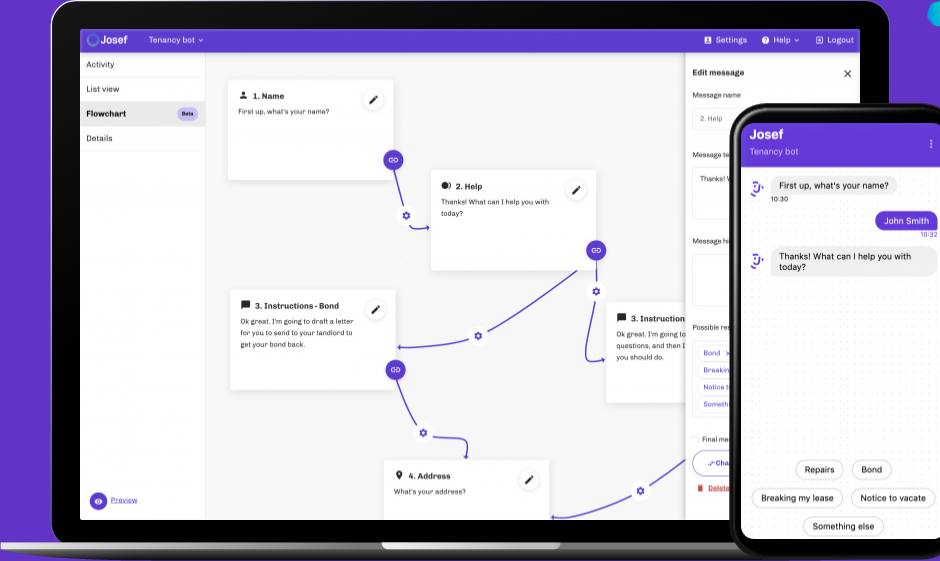
\includegraphics[scale=0.4]{images/3/chatbot-josef}
%     \caption{Ejemplo de una aplicación desarrollada en Josef}
%     \label{fig:josef}
% \end{figure}
    
% También existe TARS. (\url{https://hellotars.com/chatbot-templates/}). Es una herramienta de publicidad y marketing para construir chatbots en landing pages. Su propósito es proporcionar un aumento en la experiencia a posibles clientes mediante una conversación en lugar de contenido estático que debe ser leído. Sin embargo, esta herramienta proporciona plantillas que se pueden personalizar para cierto tipo de servicio; por ejemplo, se puede utilizar para proporcionar asesoría relacionada a la salud y terapia. La plantilla se puede utilizar para los pacientes que sufren depresión y ansiedad, manteniendo al tanto a su doctor de los síntomas que va presentando. Esto agiliza la recolección de información suficiente para los pacientes y transmite información preventiva en caso de requerir ayuda inmediata.

% \begin{figure}[ht]
%     \centering
%     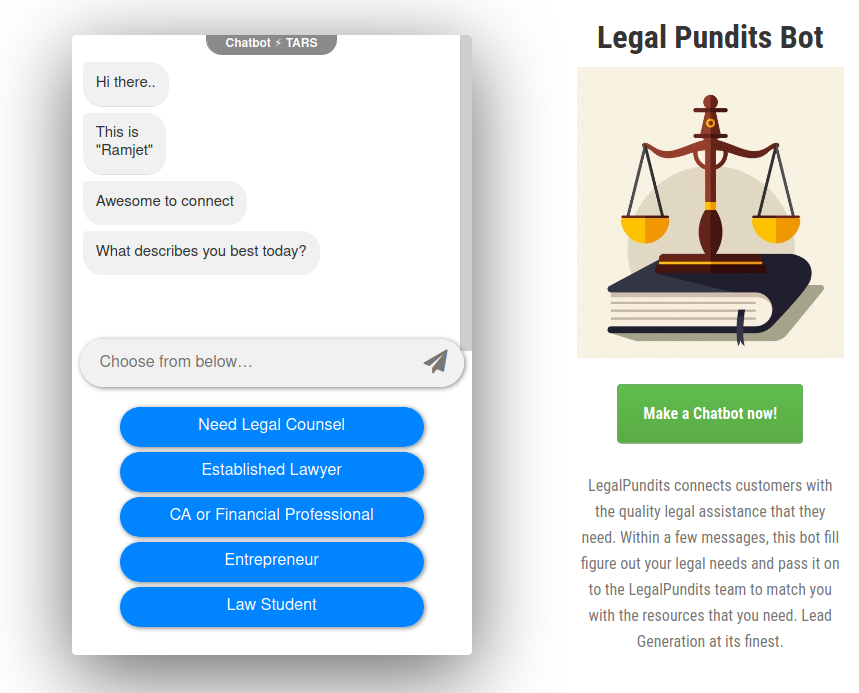
\includegraphics[scale=0.4]{images/3/chatbot-tars}
%     \caption{Plantilla de desarrollo de TARS}
%     \label{fig:tars}
% \end{figure}
    
% HaRi-Bot (\url{https://www.humanresourcesintelligence.com/}) es un chatbot desarrollado para la automatización de las operaciones de los departamentos de recursos humanos de una empresa. El objetivo de este software es el de reducir el tiempo que le toma al departamento de recursos humanos atender preguntas de los empleados, que podrían tomar desde días hasta una semana. HaRi-Bot ayuda a resolver esas que podrían consistir desde políticas internas de la empresa o en procesos administrativos.  

% \section{Librerías y APIs Para Desarrollo de Chatbots}

% Una alternativa atractiva es el de \textbf{Dialogflow} \url{https://dialogflow.com/}, el cual es un API proporcionado por Google para el desarrollo de aplicaciones que usen procesamiento de lenguaje natural. Sin embargo, depende mucho del servicio de \textbf{Google Cloud Platform}, por lo que no permitirá escalar el proyecto sin tener que considerar siempre la oferta de servicios de nube de un solo proveedor.

\section{Librerías y APIs Para Desarrollo de Chatbots}

La necesidad de automatizar un chatbot requiere que se resuelva lo siguiente:

\begin{itemize}
    \item Se debe estructurar bien el formato del conocimiento que el chatbot utiliza.
    \item La manera en que el proceso se lleva a cabo es demasiado específico al problema a resolver.
\end{itemize}

Se puede concluir entonces con estos puntos que para poder cumplir con el objetivo en mente, es necesario desarrollar una aplicación cuya solución esté a la medida del objetivo: el de informar acerca de los reglamentos del Instituto Politécnico Nacional. El estado del arte actual de aplicaciones no están enfocadas con el objetivo de este proyecto.

Es por eso que se hará énfasis en el estado de arte de tecnologías que hacen posible la construcción de chatbots: un conjunto de herramientas para el desarrollo de aplicaciones que implementen algoritmos de inteligencia artificial con filosofía \textit{open source} y licencia abierta. 

Esto permite una gran libertad en el desarrollo de ideas que tengan un impacto benéfico para la comunidad politécnica de la ESCOM; sobre todo la capacidad de poder reclamar el producto final para el bien que se vea conveniente.

Para ello, se presentan a continuación el conjunto de herramientas que ayudan a construir asistentes virtuales:

\begin{figure}[ht]
    \centering
    \begin{tabular}{c c}
        
\includegraphics[scale=0.7]{images/3/python.png} & 
\includegraphics[scale=0.5]{images/3/rasa.png} \\
        
\includegraphics[scale=0.2]{images/3/spacy.png} & 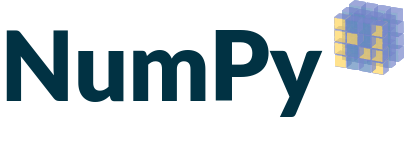
\includegraphics[scale=0.5]{images/3/numpy.png}
    \end{tabular}
    \caption{Herramientas de desarrollo open source.}
    \label{fig:open-source}
\end{figure}

\subsection{Python}

Un lenguaje de programación de alto nivel que ha tenido una alza de popularidad de uso en áreas como cómputo científico, inteligencia artificial y desarrollo web. Tiene una comunidad extensa, por lo que continuamente existe soporte para el desarrollo de aplicaciones que requieran soporte a largo plazo.

\subsection{Rasa SDK}

Desarrollado y proporcionado por una organización, quienes ofrecen servicios de desarrollo de aplicaciones para asistentes virtuales como chatbots, Rasa SDK es un kit de desarrollo de software (o SDK por sus siglas en inglés) de código abierto soportado por la organización Rasa y la comunidad abierta de desarrolladores.

Facilita la tarea de diseño conversacional con métodos de machine learning, al igual que la integración a servicios web que funcionen como canales de comunicación. Esto con el propósito que el chatbot no solo usarse en un cliente específico como una página web, sino que se pueda integrar a servicios externos como \textit{Facebook Messenger} o \textit{Slack}.

\subsection{Spacy}

Spacy es una biblioteca de funcionalidades dedicadas al procesamiento de lenguaje natural. Contiene algoritmos para procesar texto así como modelos lingüisticos complejos para varios idiomas, entre ellos el español. Su forma de poder procesar texto permite facilmente enfocarse a la lógica de algoritmos de procesamiento de lenguaje natural quitando el peso de encima de procesar cadenas de texto.


\subsection{Numpy}

Esta biblioteca proporciona un conjunto de funciones que optimizan el manejo de memoria para colecciones de datos. Esto es especialmente útil cuando esas colecciones son grandes y requiere computo extenso. Las optimizaciones sobre memoria y el procesamiento sobre ella ha encontrado sus usos en cálculo de operaciones vectoriales y matriciales.